\chapter{Completed Work}
\label{chapter:prev}
%TODO: Add in other algorithm blocks and pictures from CHRONUS paper

In this chapter, we will cover our completed research.
Our research has focused on novel implementation ]and Distributed Hash Tables (DHTs).
We have implemented and created an entirely new DHT called VHash \cite{vhash}, implemented MapReduce on Chord \cite{chordreduce}, and performed an analysis on an attack on DHTs.


\section{VHash}
DHTs all seek to minimize lookup time for their respective topologies.
This is done by minimizing the number of overlay hops needed for a lookup operation.
This is a good approximation for minimizing the latency of lookups, but does not actually do so.
Furthermore, a network might need to minimize some arbitrary metric, such as energy consumption.

VHash is a multi-dimensional DHT that minimizes routing over some given metric.
It uses a fast approximation of a Delaunay Triangulation to compute the Voronoi tessilation of a multi-dimensional space.
%Approximated routing tables



Arguably all Distributed Hash Tables (DHTs) are built on the concept of Voronoi tessellation.
In all DHTs, a node is responsible for all points in the overlay to which it is the ``closest'' node.
Nodes are assigned a key as their location in some keyspace, based on the hash of certain attributes.
Normally, this is just the hash of the IP address (and possibly the port) of the node \cite{chord} \cite{kademlia} \cite{can} \cite{pastry}, but other metrics such as geographic location can be used as well \cite{ratnasamy2002ght}.

These DHTs have carefully chosen metric spaces such that these regions are very simple to calculate.
For example, Chord \cite{chord} and similar ring-based DHTs \cite{symphony} utilize a unidirectional, one-dimensional ring as their metric space, such that the region for which a node is responsible is the region between itself and its predecessor.

Using a Voronoi tessellation in a DHT generalizes this design.
Nodes are Voronoi generators at a position based on their hashed keys.
These nodes are responsible for any key that falls within its generated Voronoi region.

Messages get routed along links to neighboring nodes.
This would take $O(n)$ hops in one dimension.
In multiple dimensions, our routing algorithm (Algorithm \ref{alg:lookup}) is extremely similar to the one used in Ratnasamy et al.'s Content Addressable Network (CAN) \cite{can}, which would be $O(n^{\frac{1}{d}})$ hops.


\begin{algorithm}
	\caption{Lookup in a Voronoi-based DHT}
	\label{alg:lookup}
	\begin{algorithmic}[1]
		\State Given node $n$
		\State Given $m$ is a message addressed for $loc$
		\State $potential\_dests \leftarrow n \cup n.short\_peers \cup n.long\_peers$
		\State $c \leftarrow $ node in $ potential\_dests$ with shortest distance to $loc$
		\If{$c$ == $n$}
			\State \Return $n$
		\Else
			\State \Return $c.lookup(loc)$
		\EndIf
	\end{algorithmic}
\end{algorithm}


Efficient solutions, such as Fortune's sweepline algorithm \cite{fortune1987sweepline}, are not usable in spaces with 2 more dimensions.
As far as we can tell, there is no way efficient to generate higher dimension Voronoi tessellations, especially in the distributed Churn-heavy context of a DHT.
Our solution is the Distributed Greedy Voronoi Heuristic.

\subsection*{Distributed Greedy Voronoi Heuristic}
A Voronoi tessellation is the partition of a space into cells or regions along a set of objects $O$, such that all the points in a particular region are closer to one object than any other object.
We refer to the region owned by an object as that object's Voronoi region.
Objects which are used to create the regions are called Voronoi generators.
In network applications that use Voronoi tessellations, nodes in the network act as the Voronoi generators.

The Voronoi tessellation and Delaunay triangulation are dual problems, as an edge between two objects in a Delaunay triangulation exists if and only if those object's Voronoi regions border each other.
This means that solving either problem will yield the solution to both.
An example Voronoi diagram is shown in Figure \ref{voro-ex}.
For additional information, Aurenhammer \cite{voronoi} provides a formal and extremely thorough description of Voronoi tessellations, as well as their applications.


\begin{figure}
	\centering
	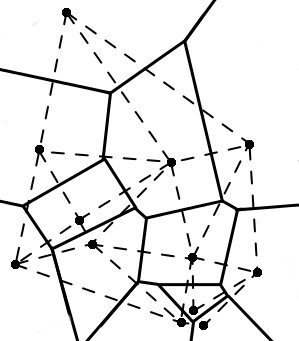
\includegraphics[width=0.5\linewidth]{figs/voronoi}
	\caption{An example Voronoi diagram for objects on a 2-dimensional space.  The black lines correspond to the borders of the Voronoi region, while the dashed lines correspond to the edges of the Delaunay Triangulation.}
	\label{voro-ex}
\end{figure}




The Distributed Greedy Voronoi Heuristic (DGVH) is a fast method for nodes to define their individual Voronoi region (Algorithm \ref{alg:dgvh}).
This is done by selecting the nearby nodes that would correspond to the points connected to it by a Delaunay triangulation.
The rationale for this heuristic is that, in the majority of cases, the midpoint between two nodes falls on the common boundary of their Voronoi regions.

%In addition, nodes should only have to compute their own Voronoi region, and possibly estimate those of its neighbors.
%Anything else is a waste of processing power.



\begin{algorithm} % make smaller
	\caption{Distributed Greedy Voronoi Heuristic}
	\label{alg:dgvh}
	\begin{algorithmic}[1]  % the numberis how many lines
		\State Given node $n$ and its list of $candidates$.
		\State Given the minimum $table\_size$
		\State $short\_peers \leftarrow$ empty set that will contain $n$'s one-hop peers
		\State $long\_peers \leftarrow$ empty set that will contain $n$'s two-hop peers
		\State Sort $candidates$ in ascending order by each node's distance to $n$
		\State Remove the first member of $candidates$ and add it to $short\_peers$
		\ForAll{$c$ in $candidates$}
		\State $m$ is the midpoint between $n$ and $c$
		\If{Any node in $short\_peers$ is closer to $m$ than $n$}
		\State Reject $c$ as a peer
		\Else
		\State Remove $c$ from $candidates$
		\State Add $c$ to $short\_peers$
		\EndIf
		\EndFor
		\While{$|short\_peers| < table\_size$ \textbf{and} $|candidates| >0$}
		\State Remove the first entry $c$ from $candidates$
		\State Add $c$ to $short\_peers$
		\EndWhile
		\State Add $candidates$ to the set of $long\_peers$
		\If{$|long\_peers| > table\_size^2$}
		\State $long\_peers \leftarrow$ random subset of $long\_peers$ of size $table\_size^2$
		\EndIf
	\end{algorithmic}
\end{algorithm}


During each cycle, nodes exchange their peer lists with a current neighbor and then recalculate their neighbors.
A node combines their neighbor's peer list with its own to create a list of candidate neighbors.
This combined list is sorted from closest to furthest.
A new peer list is then created starting with the closest candidate.
The node then examines each of the remaining candidates in the sorted list and calculates the midpoint between the node and the candidate.
If any of the nodes in the new peer list are closer to the midpoint than the candidate, the candidate is set aside.
Otherwise the candidate is added to the new peer list.


DGVH never actually solves for the actual polytopes that describe a node's Voronoi region.
This is unnecessary and prohibitively expensive \cite{raynet}.
Rather, once the heuristic has been run, nodes can determine whether a given point would fall in its region.

Nodes do this by calculating the distance of the given point to itself and other nodes it knows about.
The point falls into a particular node's Voronoi region if it is the node to which it has the shortest distance.
This process continues recursively until a node determines that itself to be the closest node to the point.
Thus, a node defines its Voronoi region by keeping a list of the peers that bound it.



\subsubsection{Algorithm Analysis}

DVGH is very efficient in terms of both space and time.
Suppose a node $n$ is creating its short peer list from $k$ candidates in an overlay network of $N$ nodes.
The candidates must be sorted, which takes $O(k\cdot\lg(k))$ operations.
Node $n$ must then compute the midpoint between itself and each of the $k$ candidates.
Node $n$ then compares distances to the midpoints between itself and all the candidates.
This results in a cost of

\[ k\cdot\lg(k) + k \text{ midpoints}  + k^{2} \text{ distances} \]


Since $k$ is  bounded by $\Theta(\frac{\log N}{\log \log N} )$ \cite{bern1991expected} (the expected maximum degree of a node), we can translate the above to

\[O(\frac{\log^{2} N}{\log^{2} \log N} )\]

In the vast majority of cases, the number of peers is equal to the minimum size of \textit{Short Peers}.
This yields $k=(3d+1)^{2}+3d+1$ in the expected case, where the lower bound and expected complexities are $\Omega(1)$.



\subsection{Experimental Results}
We evaluated the effectiveness of VHash and DGVH in creating a set of experiments.\footnote{Our results are pulled directly from \cite{dgvh} and \cite{vhash}.}
The first experiment showed how VHash could use DGVH to create a routing mesh.
Our second showed how optimizing for latency yielded better results than optimizing for least hops.

\subsubsection{Convergence}
Our first experiment examined how DGVH could be used to create a routing overlay and how well it performed in this task.
The simulation demonstrated how DGVH  formed a stable overlay from a chaotic starting topology after a number of cycles.
We compared our results to those in RayNet \cite{raynet}.
The authors of Raynet proposed a random $k$-connected graph would be a challenging initial configuration for showing a DHT relying on a gossip mechanism could converge to a stable topology.

In the initial two cycles of the simulation, each node bootstrapped its short peer list by appending 10 nodes, selected uniformly at random from the entire network.
In each cycle, the nodes gossiped , swapping peer list information.
They then ran DGVH using the new information.
We calculated the hit rate of successful lookups by simulating 2000 lookups from random nodes to random locations, as described in Algorithm \ref{alg:routesim}.
A lookup was considered successful if the network was able to determine which Voronoi region contained a randomly selected point.

Our experimental variables for this simulation were the number of nodes in the DGVH generated overlay and the number of dimensions.
We tested network sizes of 500, 1000, 2000, 5000, and 10000 nodes each in 2, 3, 4, and 5 dimensions.
The hit rate at each cycle is $\frac{hits}{2000}$, where $hits$ are the number of successful lookups.




\begin{algorithm}
	\caption{Routing Simulation Sample}
	\label{alg:routesim}
	\begin{algorithmic}[1]  % the number is how many
		\State $start \leftarrow$ random node
		\State$dest \leftarrow$ random set of coordinates
		\State $ans \leftarrow$ node closest to $dest$
		\If {$ans == start.lookup(dest)$}
		\State increment $hits$
		\EndIf
	\end{algorithmic}
\end{algorithm}

The results of our simulation are shown in Figures \ref{fig:conv2}, \ref{fig:conv3}, \ref{fig:conv4}, and \ref{fig:conv5}.
Our graphs show that a correct overlay was quickly constructed from a random configuration and that our hit rate reached 90\% by cycle 20, regardless of the number of dimensions.
Lookups consistently approached a hit rate of 100\% by cycle 30.
In comparison, RayNet's routing converged to a perfect hit rate at around cycle 30 to 35 \cite{raynet}.
As the network size and number of dimensions each increase, convergence slows, but not to a significant degree.

\begin{figure*}
	\label{fig:conv}
	\centering
	\begin{tabular}{cc}

		\begin{subfigure}{0.5\columnwidth}
			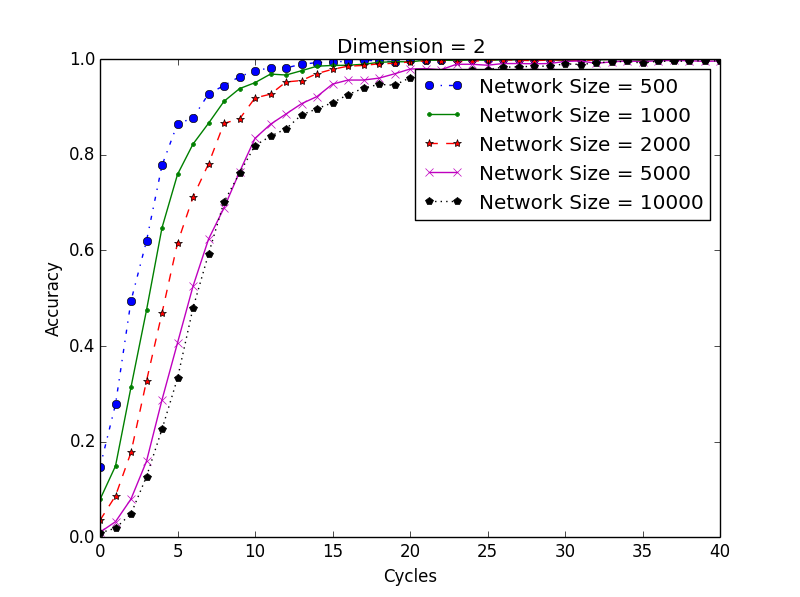
\includegraphics[width=\linewidth]{figs/conv_d2}
			\caption{This plot shows the accuracy rate of lookups on a 2-dimensional network as it self-organizes.}
			\label{fig:conv2}
		\end{subfigure} &

		\begin{subfigure}{0.5\columnwidth}
			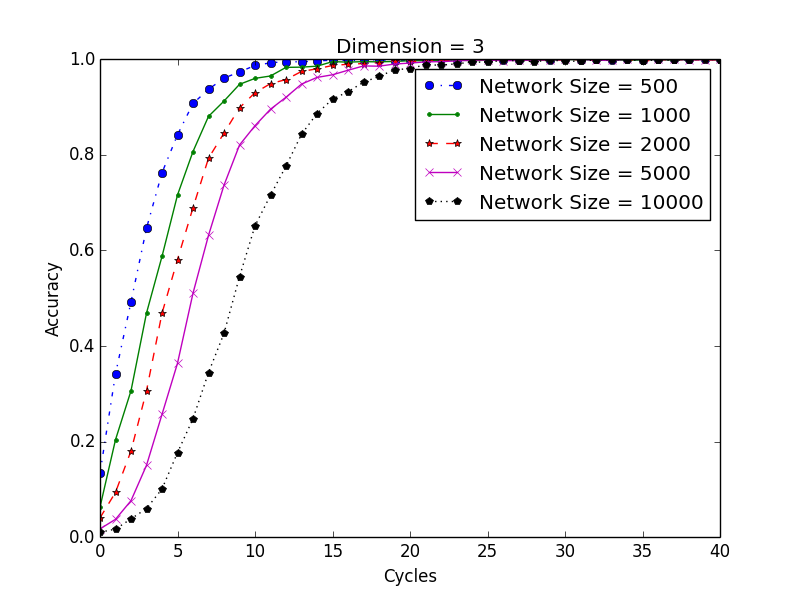
\includegraphics[width=\linewidth]{figs/conv_d3}
			\caption{This plot shows the accuracy rate of lookups on a 3-dimensional network as it self-organizes.}
			\label{fig:conv3}
		\end{subfigure} \\

		\begin{subfigure}{0.5\columnwidth}
			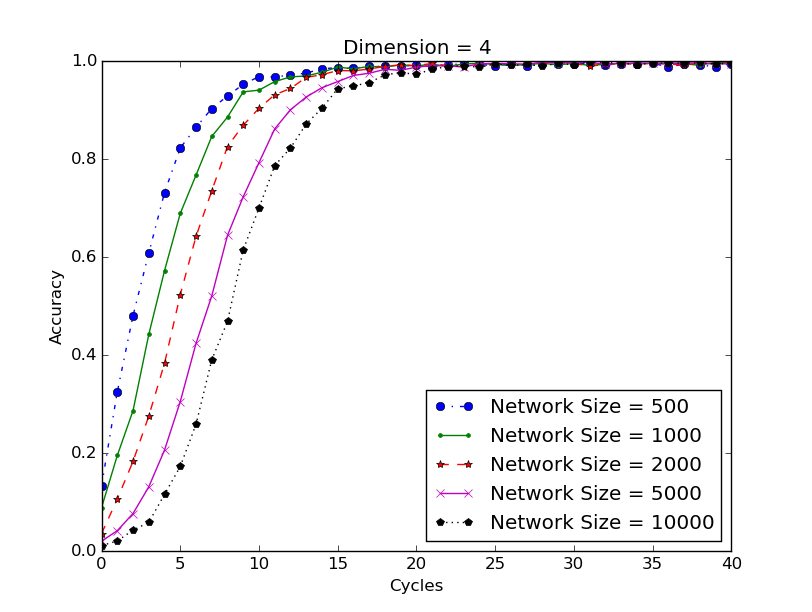
\includegraphics[width=\linewidth]{figs/conv_d4}
			\caption{This plot shows the accuracy rate of lookups on a 4-dimensional network as it self-organizes.}
			\label{fig:conv4}
		\end{subfigure} &


		\begin{subfigure}{0.5\columnwidth}
			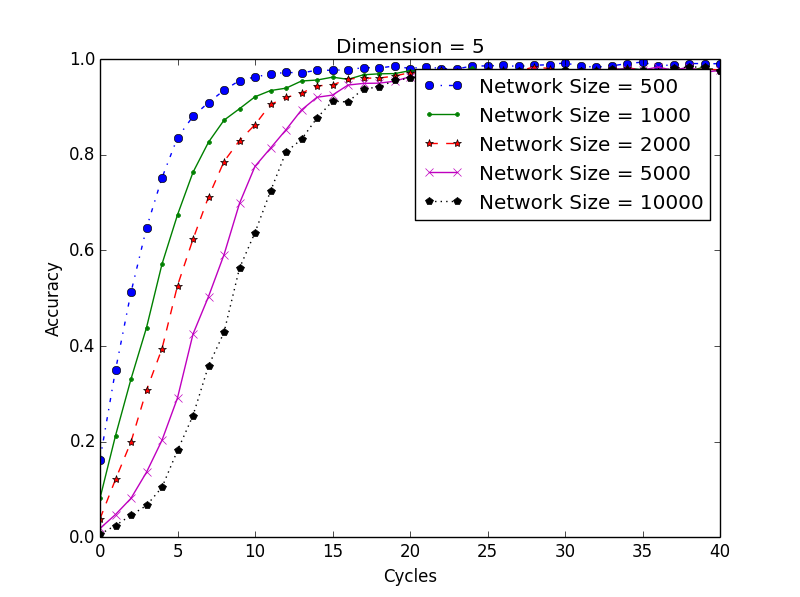
\includegraphics[width=\linewidth]{figs/conv_d5}
			\caption{This plot shows the accuracy rate of lookups on a 5-dimensional network as it self-organizes.}
			\label{fig:conv5}
		\end{subfigure}

	\end{tabular}
	\caption{These figures show that, starting from a randomized network, DGVH forms a stable and consistent network topology.
		The Y axis shows the success rate of lookups and the X axis show the number of gossips that have occurred.
		Each point shows the fraction of 2000 lookups that successfully found the correct destination.}

\end{figure*}

\subsubsection{Latency Distribution Test}
The goal of our second set of experiments was to demonstrate VHash's ability to optimize a selected network metric: latency in this case.
In our simulation, we used the number of hops on the underlying network as an approximation of latency.
We compared VHash's performance to Chord \cite{chord}.
As we discussed in Chapter \ref{chapter:background} Chord is a well established DHT with an $O(\log(n))$ sized routing table and $O(\log(n))$ lookup time measured in overlay hops.

Instead of using the number of hops on the overlay network as our metric, we are concerned with the actual latency lookups experience traveling through the \emph{underlay} network, the network upon which the overlay is built.
Overlay hops are used in most DHT evaluations as the primary measure of latency.
It is the best approach available when there are no means of evaluating the characteristics of the underlying network.
VHash is designed with a capability to exploit the characteristics of the underlying network.
With most realistic network sizes and structures, there is substantial room for latency reduction in DHTs.

For this experiment, we constructed scale free network with 10000 nodes placed at random (which has an approximate diameter of 3 hops) as an underlay network \cite{cohen2000resilience} \cite{pastor2001epidemic} \cite{hagberg2004}.
We chose to use a scale-free network as the underlay, since  scale free networks model the Internet's topology \cite{cohen2000resilience} \cite{pastor2001epidemic}.
We then chose a random subset of nodes to be members of the overlay network.
Our next step was to measure the distance in underlay hops between 10000 random source-destination pairs in the overlay.
VHash generated an embedding of the latency graph utilizing a distributed force directed model, with the latency function defined as the number of underlay hops between it and its peers.

Our simulation created 100, 500, and 1000 node overlays for both VHash and Chord.
We used 4 dimensions in VHash and a standard 160 bit identifier for Chord.




\begin{figure}

\begin{subfigure}{\columnwidth}
\centering
	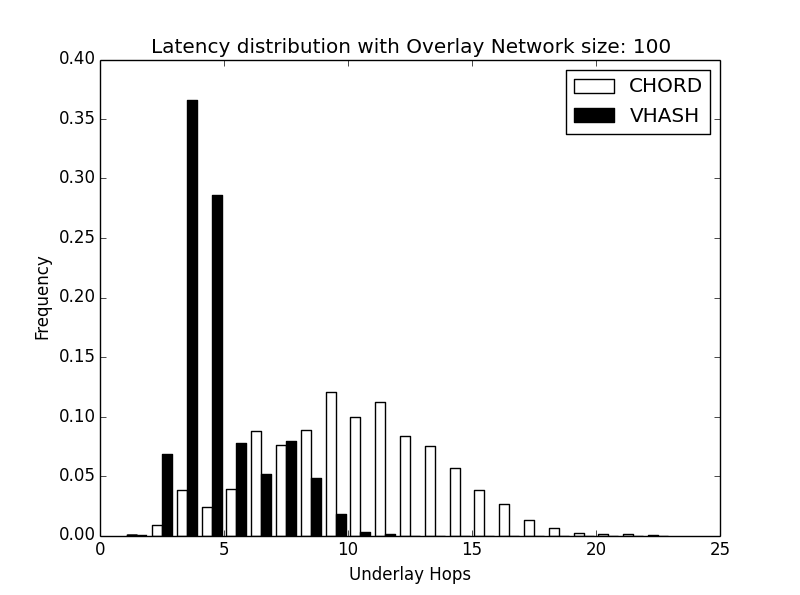
\includegraphics[width=0.5\linewidth]{figs/hist_100}
	\caption{Frequency of path lengths on Chord and VHash in a 100 node overlay.}
	\label{fig:hist100}
\end{subfigure}

\begin{subfigure}{\columnwidth}
	\centering
	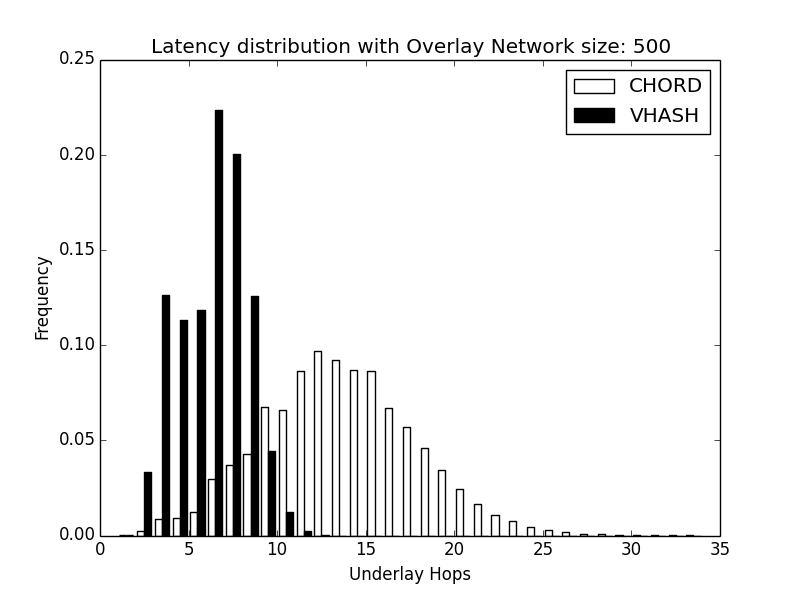
\includegraphics[width=0.5\linewidth]{figs/hist_500}
	\caption{Frequency of path lengths on Chord and VHash in a 500 node overlay.}
	\label{fig:hist500}
\end{subfigure}

\begin{subfigure}{\columnwidth}
	\centering
	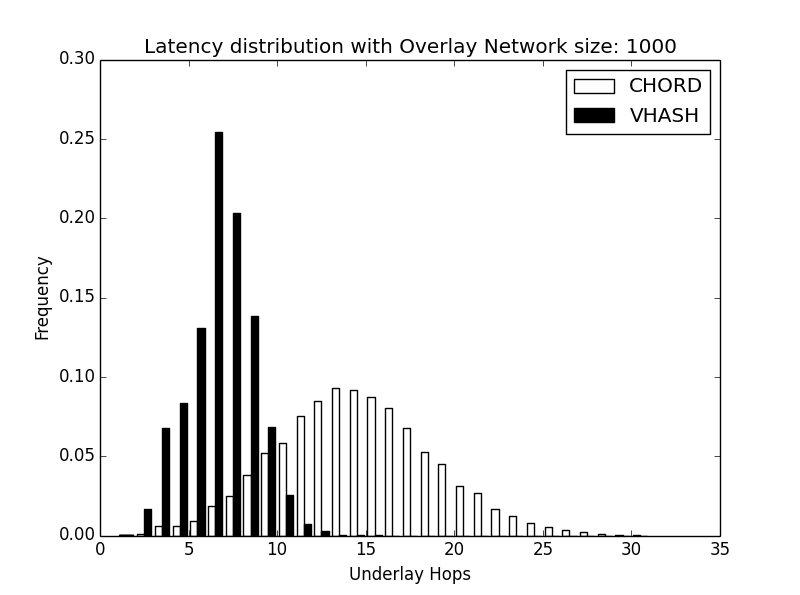
\includegraphics[width=0.5\linewidth]{figs/hist_1000}
	\caption{Frequency of path lengths on Chord and VHash in a 1000 node overlay.}
	\label{fig:hist1000}
\end{subfigure}

\caption{Figures \ref{fig:hist100}, \ref{fig:hist500}, and \ref{fig:hist1000} show the difference in the performance of Chord and VHash for 10,000 routing samples on a 10,000 node underlay network for differently sized overlays.
The Y axis shows the observed frequencies and the X axis shows the number of hops traversed on the underlay network.
VHash consistently requires fewer hops for routing than Chord.}
\end{figure}




Figures \ref{fig:hist100}, \ref{fig:hist500}, and \ref{fig:hist1000} show the distribution of path lengths measured in underlay hops in both Chord and VHash.
VHash significantly outperformed Chord and considerably reduced the underlay path lengths in three network sizes.

We also sampled the lookup length measured in overlay hops for a 1000 sized Chord and VHash network.
As seen in Figure \ref{fig:histover}, the paths measured in overlay for VHash were significantly shorter than those in Chord.
In comparing the overlay and underlay hops, we find that for each overlay hop in Chord, the lookup must travel 2.719 underlay hops on average; in VHash, lookups must travel 2.291 underlay hops on average for every overlay hop traversed.

Recall that this work is based on scale free networks, where latency improvements are difficult.
An improvement of 0.4 hops over a diameter of 3 hops is significant.
VHash has on average less overlay hops per lookup than Chord, and for each of these overlay hops we consistently traverse more efficiently across the underlay network.
\begin{figure}[h]
	\centering
	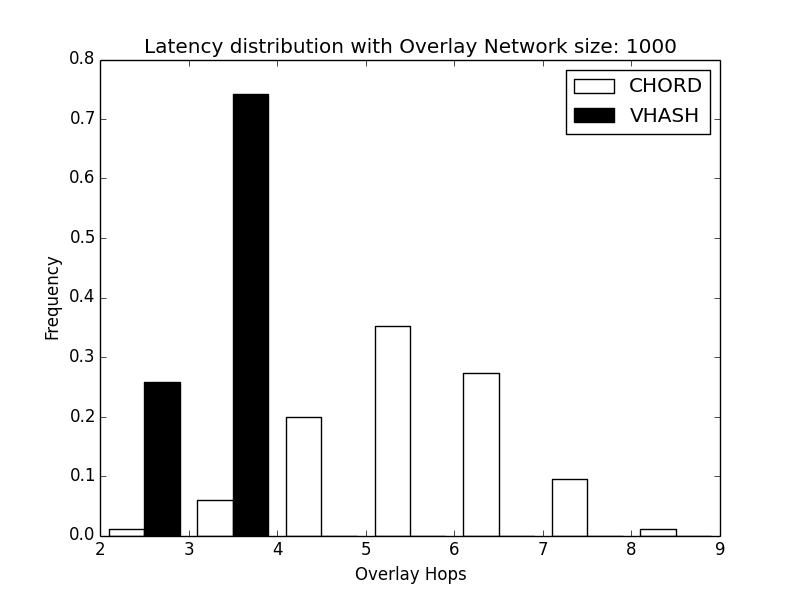
\includegraphics[width=\linewidth]{figs/hist_overlay_4d}
	\caption{Comparison of Chord and VHash in terms of overlay hops.  Each overlay has 1000 nodes.  The Y axis denotes the observed frequencies of overlay hops and the X axis corresponds to the path lengths in overlay hops.}
	\label{fig:histover}
\end{figure}




\subsection{Remarks}

Voronoi tessellations have a wide potential for applications in ad-hoc networks, massively multiplayer games, P2P, and distributed networks.
However, centralized algorithms for Voronoi tessellation and Delaunay triangulation are not applicable to decentralized systems.
In addition, solving Voronoi tessellations in more than 2 dimensions is computationally expensive.

We created a distributed heuristic for Voronoi tessellations in an arbitrary number of dimensions.
Our heuristic is fast and scalable, with a expected memory cost of $(3d+1)^{2}+3d+1$ and expected maximum runtime of O$(\frac{\log^{2} N}{\log^{2} \log N} )$.

We ran two sets of experiments to demonstrate VHash's effectiveness.
Our first set of experiments demonstrated that our heuristic is reasonably accurate  and our second set demonstrates that reasonably accurate is sufficient to build a P2P network which can route accurately.
Our second experiment showed that VHash  could significantly reduced the latency in Distributed Hash Tables.

%Our next step is to create a formal protocol and implementation for a Voronoi tessellation-based distributed hash table using DGVH.
%We can use this DHT to choose certain metrics we want to measure, such as latency, or trust, and embed that information as part of a node's identity.
%By creating an appropriate distance measurement, we can route along some path that minimizes or maximizes the desired metric.
%Rather than create an overlay that minimizes hops, we can have our overlay minimize latency, which is the actual goal of most routing algorithms.

%\subsection*{Peerlist and Topology}
%Like CAN \cite{can}, VHash tracks only neighbors for it's peers.
%We enforce a lower limit on the size of the peerlist to avoid nodes being


%\subsection*{Joining}


%\subsection*{Fault Tolerance}




\section{ChordReduce}
DHTs have received a great deal of research due to their popularity as the backbone for structured P2P system primarily used for file-sharing.
There are two recent and fairly open questions that we want to examine.

\begin{enumerate}
	\item How and in what contexts  can DHTs effectively be used for distributed computations?
	\item How can nodes in a DHT autonomously detect and redistribute imbalances in the network load?
\end{enumerate}

This section will talk about ChordReduce, in which we have made preliminary attempts to answer the first question by implementing MapReduce on a DHT.
The next section, Section \ref{sec:auto-load-bal}, discusses the our preliminary work in answering the second.

\subsection{Background and Motivation}

Distributed computing is a current trend and will continue to be the approach for intensive  applications.
We see this in the development of cloud computing \cite{p2p-cloud}, volunteer computing frameworks like BOINC \cite{anderson2004boinc} and Folding@Home \cite{larson2002folding},and MapReduce  \cite{mapreduce}.
Google's MapReduce  in particular has rapidly become an integral part in the world of data processing.
A user can use MapReduce to take a large problem, split it into small, equivalent tasks and send those tasks to other processors for computation.
The results are sent back to the user and combined into one answer.

Popular platforms for MapReduce, such as Hadoop \cite{hadoop}  \cite{shvachko2010hadoop}, are explicitly designed to be used in large datacenters \cite{hadoopAssumptions} and the majority of research has been focused there.
However, as we have previously mentioned, there are notable issues with a centralized design.

First and foremost is the issue of fault-tolerance.
Centralized designs have a single point of failure \cite{shvachko2010hadoop}.
So long as all computing resources are located in one geographical area or rely on a particular node, a power outage or catastrophic event could interrupt computations or otherwise disrupt the platform \cite{babaoglu2014people}.

A centralized design assumes that the network is relatively unchanging and may not have mechanisms to handle node failure during execution or, conversely, cannot speed up the execution of a job by adding additional workers on the fly.
Many environments also anticipate a certain degree in homogeneity in the system.
Finally deploying these systems and developing programs for them has an extremely steep learning curve.

There is no reason that these assumptions need to be the case for MapReduce, or for many distributed computing frameworks in general.
Moving away from the data center context opens up more possibilities for distributed computing, such as P2P clouds \cite{p2p-cloud}.
However, without a centralized framework, the network needs some kind of protocol to organize the various components in the network.
As part of our research, we developed a highly robust and distributed MapReduce framework based on Chord, called ChordReduce \cite{chordreduce}.

There a number of reasons to used a DHT as the protocol for a distributed computing platform.
First, nodes ID and their location in the network are strongly bound to what data they are responsible for, such that any node can lookup which node is responsible a particular piece of data.
This obviates the need for a centralized organizer to maintain this bit of metadata or assign backups for data, as nodes can do this autonomously.
DHTs assume that the network is heterogeneous, rather than homogeneous.
They have been used for over a decade for P2P file-sharing applications for these reasons.


%\subsubsection{P2P cloud}
%http://www.cs.unibo.it:443/pub/TR/UBLCS/2011/2011-10.pdf

%Clouds and Volunteer Computing platforms are different.
%Clouds@home
%Nanodatacenter

\subsection{What is ChordReduce?}

ChordReduce is designed as a more abstract framework for MapReduce, able to run on any arbitrary distributed configuration.
ChordReduce leverages the features of distributed hash tables to handle distributed file storage, fault tolerance, and lookup.
We designed ChordReduce to ensure that no single node is a point of failure and that there is no need for any node to coordinate the efforts of other nodes during processing.



\subsubsection{File System}
Our central design philosophy was to leverage as many features of the underlying DHT as possible.
For example, we do not need to create a new distributed file system, as we can just use the DHT to hash file identifiers and use the DHT to store the file at the node responsible for that key.

If the file is large, we can instead use Dabek et al.'s Cooperative File System or CFS \cite{CFS}.
In CFS, files are split into approximately equally sized blocks.
Each block is treated as an individual file and is assigned a key equal to the hash of its contents.
The block is then stored at the node responsible for that key.
The node that would normally be responsible for the whole file instead stores a \textit{keyfile}.
The keyfile is an ordered list of the keys corresponding to the files' block and is created as the blocks are assigned their respective keys.
When the user wants to retrieve a file, they first obtain the keyfile and then request each block specified in the keyfile.


\subsubsection{Computation}
ChordReduce treats each task or target computation as an object of data.
This means we can distribute them in the same manner as files and rely on the protocol to route them and provide robustness.


In ChordReduce, each node takes on responsibilities of both a worker node and master node, in the same way that a node in a P2P file-sharing service acts as both a client and a server.
A user starts a job, contacts a node at a specified hash address and provides it with the tasks.
This address can be chosen arbitrarily or be a known node in the ring.
We call this node the \textit{stager} for this particular job.

The job of the stager is to divide the work into \emph{data atoms}, the smallest units of work.
This might represent a block of text, the result of a summation for a particular intermediate value, or a subset of items to be sorted.
The specifics of how to divide the work are defined by the user in a \emph{stage} function.
The data atoms also contain user created Map and Reduce functions.

If the user wants to perform a MapReduce job on a particular file on the network, the stager locates the keyfile for the data and creates a data atom for each block in the file.
Each data atom is then sent to the node responsible for their corresponding block.
When the data atom reaches its destination node, that node retrieves the necessary data and applies the Map function.
The results are stored in a new data atom,  which are then sent back to the stager's hash address (or some other user defined address).
This will take $O(\lg n)$ hops traveling over Chord's fingers.
At each hop, the node waits a predetermined minimal amount of time to accumulate additional results (In our experiments, this was 100 milliseconds).
Nodes that receive at least two results merge them using the Reduce function.
The results are continually merged until only one remains at the hash address of the stager.


Some MapReduce jobs do not rely on a file stored on the network, such as a Monte-Carlo approximation.
In this situation, the data atoms define a task to be run multiple times.
In this case, the created data atoms are then each given a random hash and sent to the node responsible for that hash address, guaranteeing they are evenly distributed throughout the network.
From there, the execution is identical to the above scenario.


%Once the data atoms are sent out, the stager's job is done and it behaves like any other node in the network. The staging period is the only time ChordReduce is vulnerable to churn, and only if the stager leaves the ring in the middle of sending out data atoms.  The user would get some results back, but only for the data the stager managed to send out.

Once all the Reduce tasks are finished, the user retrieves the results from the node at the stager's address.
This may not be the stager himself, as the stager may no longer be in the network.
The stager does not need to collect the results himself, since the work is sent to the stager's hash address, rather than the stager itself.
Thus, the stager could quit the network after staging, and both the user and the network would be unaffected by the change.
This eliminates the need for a single specific root node and provides fault tolerance.
% Here, we are leverging two features. First, we use the automatic assignment of responsibility to automatically route the data to the sucessor.  %Second, the same process Chord uses to backup files is used to backup the intermediate data.

Similar precautions are taken for nodes working on Map and Reduce tasks.
Those tasks are backed up by a node's successor, who will run the task if the node leaves before finishing its work (e.g. the successor loses his predecessor).
The task is given a timeout by the node.
If the backup node detects that the responsible node has failed, he starts the work and backs up again to \emph{his} successor.
Otherwise, the data is tossed once the timeout expires.
This is done to prevent a job being submitted twice.

An advantage of our system is the ease of development and deployment.
The developer does not need to worry about distributing work evenly, nor does he have to worry about any node in the network going down.
The stager does not need to keep track of the status of the network.
The underlying Chord ring handles that automatically.
If the user finds they need additional processing power during runtime, they can boot up additional nodes, which would automatically be assigned work based on their hash value.
If a node goes down while performing an operation, his successor takes over for him.
This makes the system extremely robust during runtime.


\subsubsection{Robustness}
Since the system is distributed, we need to assume that any member of the network can go down at any time.
When a node fails or leaves Chord, the failed node's successor will become responsible for all of the failed nodes keys.
Likewise, each node in the ChordReduce network relies on their successor to act as a backup.

To prevent data from becoming irretrievable, each node periodically sends backups to its successor.
In order to prevent a cascade of backups of backups, the node only sends data that it is currently responsible for.
This changes as nodes enter and leave the network.
If a node's successor leaves, the node sends a backup to his new successor.
If the node fails, the successor is able to take his place almost immediately.
This scheme is used to not only backup files, but the computational tasks as well.

This procedure prevents any single node failure or sequences of failures from harming the network.
Only the failure of multiple neighboring nodes poses a threat to the network's integrity.
Recall that a node's ID in the network does not map to a geographical locations.
Any failure that affects multiple nodes simultaneously would be spread uniformly throughout the network.
This means if successive nodes to fail simultaneously, they do so independently.

Assume node has failure rate $r < 1$ and that the each node backs up their data with $s$ successive nodes downstream.
If one of these nodes fail, the next successive node takes its place and the next upstream node becomes another backup.
This ensures there will always be $s$ backups.
The integrity of the ring would only be jeopardized if $s+1$ successive nodes failed simultaneously.
The chances of this would be $r^s+1$, as each failure would be independent.


A final consequence of this is load-balancing during runtime.
When a joining node $n$ find his successor, $n$ asks if the successor is holding any data $n$ should be responsible for.
The successor looks at all the data $n$ is responsible for and sends it to $n$.
The successor maintains this data as a backup for $n$.
Because Map tasks are backed up in the same manner as data, a node can take the data and corresponding tasks he is responsible for and begin performing Map tasks immediately.

\subsection{Experiments}

We created a prototype of ChordReduce in order to demonstrate it was a viable framework.
To acheive this, we had to show ChordReduce had these three properties:
\begin{enumerate}
	\item ChordReduce provided significant speedup during a distributed job.
	\item ChordReduce scaled.
	\item ChordReduce handled churn during execution.
\end{enumerate}


We needed to demonstrate speedup by showing that a job handled by multiple workers generally finished sooner than the same job handled by a single worker.  
More formally we need to establish that $\exists n$ such that $T_{n} < T_{1}$, where $T_{n}$ is the amount of time it takes for $n$ nodes to finish the job.

To establish scalability, we needed to show that the cost of distributing the work grows logarithmically with the number of workers.  
We needed to demonstrate that the larger the job is, the more nodes can work on the problem before we begin experiencing diminishing returns. 
This can be stated as $$T_{n} = \frac{T_{1}}{n} + k \cdot \log_{2}(n)$$, where $\frac{T_{1}}{n}$ is the amount of time the job would take when distributed in an ideal universe and $k \cdot \log_{2}(n)$ is network induced overhead, $k$ being an unknown constant dependent on network latency and available processing power.

Finally, to demonstrate robustness, we had to show that ChordReduce can handle arbitrary node failure in the ring and that such failures minimally impacted the overall speed of computation

\subsubsection{Setup}


To stress test our framework, we ran a Monte-Carlo approximation of $\pi$. 
This process is analogous to having a square containing  the top-right quadrant of a circle (Fig. \ref{fig:dartboard}), and then throwing darts at random locations.  
Counting the ratio of darts that land inside the circle to the total number of throws yields an approximation of $\frac{\pi}{4}$.  
The more darts we throw, i.e. the more samples that are taken, the more accurate the approximation.\footnote{This is not and was not intended to be a particularly good approximation of $\pi$.
Each additional digit of accuracy requires increasing the number of samples taken by an order of magnitude.}


We chose this experiment for a number of reasons. 
The job is extremely easy to distribute.  
This also made it very easy to test scalability. 
By doubling the amount of samples, we can double the amount of work each node gets.  
We could also test the effectiveness of distributing the job among different numbers of workers.


\begin{figure}
	\centering
	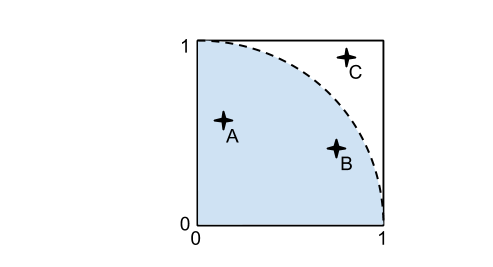
\includegraphics[width=0.5\linewidth]{figs/dartboard}
	\caption{The "dartboard." The computer throws a dart by choosing a random $x$ and $y$ between 0 and 1.  If $x^{2} + y^{2} < 1^{2} $, the dart landed inside the circle.  $A$ and $B$ are darts that landed inside the circle, while $C$ did not.}
	\label{fig:dartboard}
\end{figure}


Each Map job was defined as the number of throws the node must make and yielded total number of throws and the number of throws that landed inside the circular section.  
Reducing these results was then a matter of adding the respective fields together. 

We ran our experiments using Amazons's Elastic Compute Cloud (EC2) service.  
Amazon EC2 allows users to purchase an arbitrary amount of virtual machines by the hour. 
Each node was an individual EC2 small instance with a preconfigured Ubuntu 12.04 image.  
%These instances were capable enough to provide constant computation, but still weak enough that they would be overwhelmed by traffic on occasions, creating a constant churn effect in the ring.  

Once started, nodes retrieved the latest version of the code and run it as a service, automatically joining the network.  
We could choose any arbitrary node as the stager and tell it to run the MapReduce process. 
We found that the network was robust enough that we could take a node we wanted to be the stager out of the network, modify its MapReduce test code, have it rejoin the network, and then run the new code without any problems. 
Since only the stager had to know how to create the Map tasks, the other nodes did not have to be updated and execute the new tasks they are given.

We ran our experiments on groups of 1, 10, 20, 30, and 40 workers, which generated a $10^{8}$ sample set and a $10^{9}$ sample set.
Additionally, we gathered data on a $10^{7}$ sample set using 1, 5, 10, 20, 30 workers.  
To test churn, we ran an experiment where each node had an equal chance of leaving and joining the network and varied the level of churn over multiple runs.  

We also utilized a subroutine we wrote called $plot$, which sends a message sequentially around the ring to establish how many members there are.  
If $plot$ failed to return in under a second, the ring was experiencing structural instability.

\begin{figure}
	\centering
	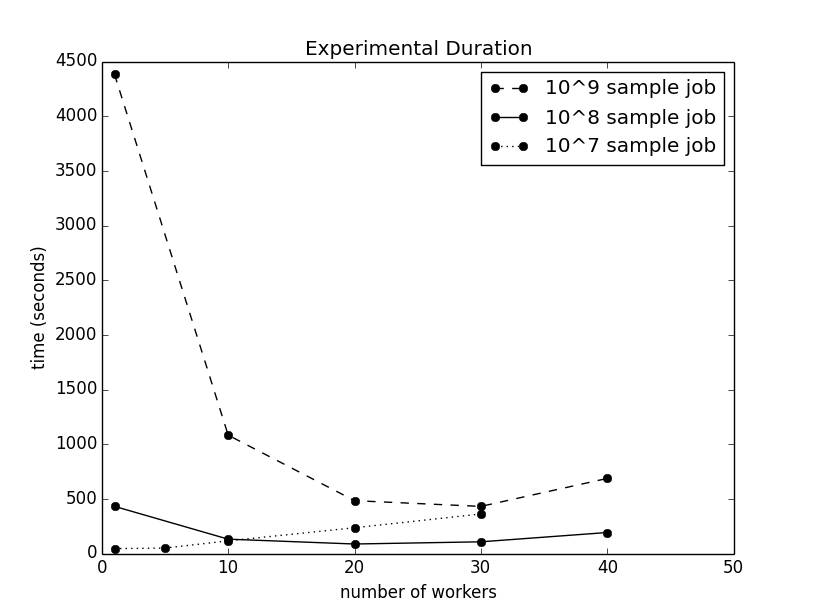
\includegraphics[width=0.5\linewidth]{figs/expTime}
	\caption{Our results show that for a sufficiently large job, it was almost always preferable to distribute it.  
		When the job is too small, such as with the $10^{7}$ data set, our runtime is dominated by the overhead.  
		Our results are what we would expect when overhead grows logarithmically to the number of workers.}
	\label{fig:expTime}
\end{figure}


\begin{figure}
	\centering
	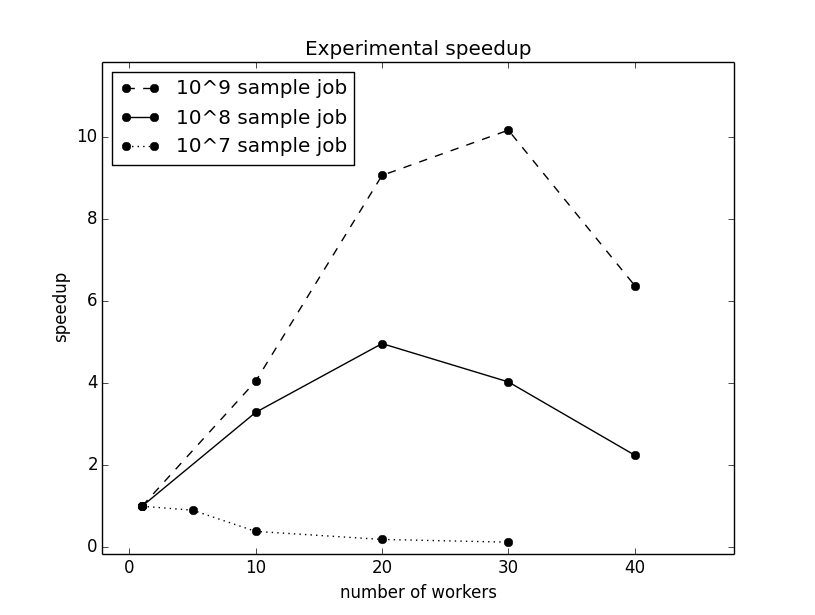
\includegraphics[width=0.5\linewidth]{figs/expSpeed}
	\caption{The larger the size of the job, the greater the gains of distributing with ChordReduce.  In addition, the larger the job, the more workers can be added before we start seeing diminishing returns.  This demonstrates that ChordReduce is scalable.}
	\label{fig:expSpeed}
\end{figure}

Fig. \ref{fig:expTime} and Fig. \ref{fig:expSpeed} summarize the experimental results of job duration and speedup.  
Our default series was the $10^{8}$ samples series.  
On average, it took a single node 431 seconds, or approximately 7 minutes, to generate $10^{8}$ samples.  
Generating the same number of samples using ChordReduce over 10, 20, 30, or 40 nodes was always quicker.  
The samples were generated fastest when there were 20 workers, with a speedup factor of 4.96, while increasing the number of workers to 30 yielded a speedup of only 4.03.  
At 30 nodes, the gains of distributing the work were present, but the cost of overhead ($k \cdot \log_{2}(n)$) had more of an impact.  
This effect is more pronounced at 40 workers, which experienced  a speedup of only 2.25.

Since our data showed that approximating $\pi$ on one node with $10^{8}$ samples took approximately 7 minutes, collecting $10^{9}$ samples on a single node would take 70 minutes at minimum.  
Fig. \ref{fig:expSpeed} shows that the $10^{9}$ set gained greater benefit from being distributed than the $10^{8}$ set, with the speedup factor at 20 workers being 9.07 compared to 4.03.  
In addition, dimishing returns only showed up at 40 workers, compared with the $10^{8}$ data set, which began its drop off at 30 workers.
This behavior showed that the larger the job being distributed, the greater the gains of distributing the work using ChordReduce.

The $10^{7}$ sample set confirms that the network overhead is logarithmic.  
At that size, it is not effective to run the job concurrently and we start seeing overheard acting as the dominant factor in runtime.  
This matches the behavior predicted by our equation, $T_{n} = \frac{T_{1}}{n} + k \cdot \log_{2}(n)$. 
For a small $T_{1}$, $\frac{T_{1}}{n}$  approaches 0 as $n$ gets larger, while $k \cdot \log_{2}(n)$, our overhead, dominates the sample.  
The samples from our data set fit this behavior, establishing that our overhead increases logarithmically with the number of workers.


\begin{figure}
	\centering
	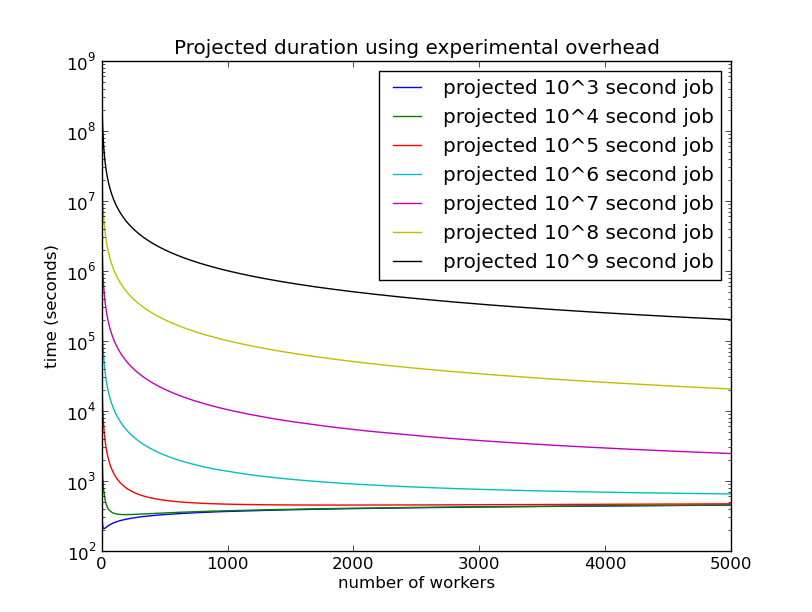
\includegraphics[width=0.5\linewidth]{figs/projTime}
	\caption{The projected runtime using ChordReduce for differently sized jobs.  Each curve projects the expected behavior for job that takes a single worker the specified amount of time.}
	\label{fig:projTime}
\end{figure}

\begin{figure}
	\centering
	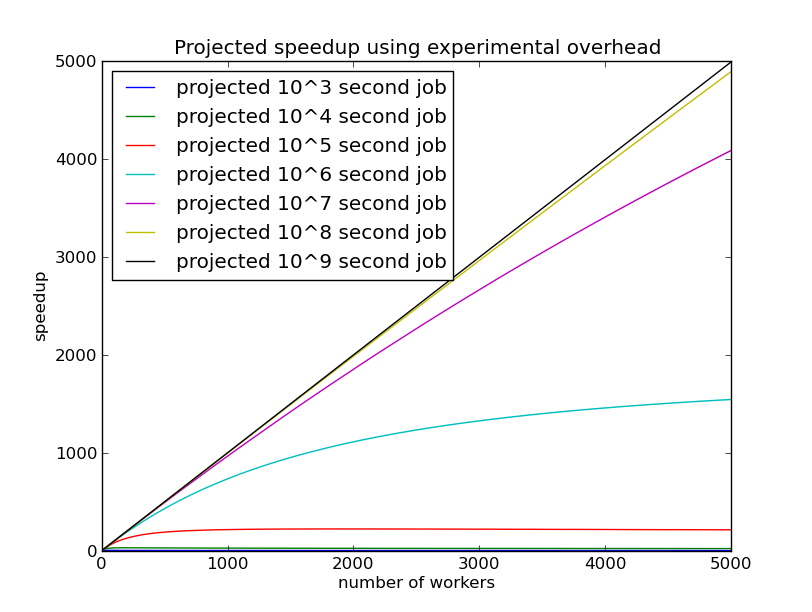
\includegraphics[width=0.5\linewidth]{figs/projSpeed}
	\caption{The projected speedup for different sized jobs. }
	\label{fig:projSpeed}
\end{figure}

Since we were able to establish that $T_{n} = \frac{T_{1}}{n} + k \cdot \log_{2}(n)$, we created an estimate how long a job that takes an arbitrary amount of time to run on a single node would take using ChordReduce.  
Our data points indicated that the mean value of $k$ for this problem was 36.5.  
Fig. \ref{fig:projTime} shows that any jobs that would take more than $10^{4}$ seconds for single worker, we can expect there would still be benefit to adding an additional worker, even when there are already 5000 workers already in the ring.  
Fig. \ref{fig:projSpeed} further emphasizes this. Note that as the jobs become larger, the expected speedup from ChordReduce  approaches linear behavior.


Table \ref{tab:churnSpeed} shows the experimental results for different rates of churn. 
We discus these experimental results and their significance in Section \ref{sec:auto-load-bal}.
\begin{table}
	\centering
	\begin{tabular}{|r|r|r|}
		\hline
		Churn rate per second & Average runtime (s) & Speedup vs 0\% churn\\ \hline{}
		0.8\% & 191.25 & 2.15 \\ \hline
		0.4\% & 329.20 & 1.25 \\ \hline
		0.025\% & 431.86 & 0.95 \\ \hline
		0.00775\%  & 445.47 & 0.92 \\ \hline
		0.00250\% & 331.80  &  1.24 \\ \hline
		0\% & 441.57 & 1.00 \\ \hline
	\end{tabular}
	\caption{}
	\label{tab:churnSpeed}
\end{table}


%These results show the system  is relatively insensitive to churn.  
%We started with 40 nodes in the ring and generated $10^{8}$ samples while experiencing different rates of churn, as specified in Table \ref{churnSpeed}.  
%At the 0.8\% rate of churn, there is a 0.8\% chance each second that any given node will leave the network followed by another node joining the network at a different location. 
%The joining rate and leaving rate being identical is not an unusual assumption to make \cite{marozzo2012p2p} \cite{load}.

%Our testing rates for churn are an order of magnitude higher than the rates used in the P2P-MapReduce simulation  \cite{marozzo2012p2p}.  In their paper, the highest rate of churn was only 0.4\% per minute. Because we were dealing with fewer nodes, we chose larger rates to demonstrate that ChordReduce could effectively handle a high level of churn.


Our experiments show that for a given problem, ChordReduce can effectively distribute the problem, yielding a substantial speedup.  
Furthermore, our results showed that the larger the problem is, the more workers could be added before diminishing returns were incurred.  
During runtime, we experienced multiple instances where $plot$ would fail to run and the stager would report socket errors, indicating that it had lost connection with a node in the ring.  Despite this turbulence, every node managed to reestablish connection with each other and report back all the data.  
This further demonstrated that we were able to handle the churn in the network.


\subsection{Heterogeneity Calculation}

One of the advantages to using homogeneous hardware is that each machine, each core, each node is the same.
To evenly distribute the workload, you just have to give each machine the same amount of work.
While a

This is more difficult in a heterogeneous system, such as ChordReduce, as each machine can shoulder a different amount of work.
How do we distribute work evenly across a heterogeneous system?

We can solve this by adjusting the amount of nodes representing each machine in the network.
Machines that can handle a larger load create more nodes in the network.
Besides solving the heterogeneous load-balancing problem, increasing the number of nodes in the system increases the overall load-balancing of the system.

The question we must answer is ``how?''
We need to create some unit of measurement for a distributed computing system and research if any other researchers have asked this problem.
Furthermore, this measurement might need to be relative to other nodes in the network, since the only basis for comparison are the scores of the peers. 
Finally, this process needs to be handled autonomously by each node.
This is part of the proposed work discussed in Chapter \ref{chapter:experiments}.
\section{Autonomous Load Balancing}
\label{sec:auto-load-bal}


During our experiments testing the capabilities of ChordReduce, we experienced a significant and completely unexpected anomaly while testing churn.
One of the things previous research \cite{marozzo2012p2p}  \cite{leemap} in the same area we felt we needed to explore better was how a completely decentralized computation could handle churn.
Now, despite our initial prototype having numerous bugs and only able to handle small networks, we were fairly certain of it's ability to handle churn.

Marozzo et al.\ \cite{marozzo2012p2p} tested their network using churn rates of 0.025\%, 0.05\%, 0.1\%, 0.2\%, and 0.4\% per minute.
The churn rate of $cr << 1$ per minute means that each minute on average, $cr \cdot n$ nodes leave the network and $cr \cdot n$  new nodes join the network.\footnote{It is standard practice to assume the joining rate and leaving rate are equal.}
This could effectively be thought of as each node flipping a weighted coin every minute.
When the coin lands on tails, the node leaves.
A similar process happens for nodes wanting to join the network.

We wanted the robustness of our system to be beyond reproach, so we tested at rates from 0.0025\% to 0.8\% \textbf{\textit{per second}}, 120 times the fastest rate used to test P2P-MapReduce.
This is an absurdly fast and unrealistic speed, the only purpose of which was to cement the fault tolerance of the system.
Since we were testing ChordReduce on Amazon's EC2 and paying per instance per hour, we limited the number of nodes.
Rather than having a pool of nodes waiting to join the network, we conserved our funds by having leaving nodes immediately rejoin the network under a new IP/port combo.
The meant our churn operation was essentially a simultaneous leave and join.


What we found was that jobs on ChordReduce finished twice as fast under the unrealistic levels churn (0.8\% per second) than no churn (Table \ref{tab:churnSpeed}).
This completely mystified us.
Churn is a disruptive force; how can it be aiding the network?

\subsection*{Hypothesis}
We hypothesize this was due to the number of data pieces (larger) vs the number of workers (smaller).
There were more workers than there were pieces of data, so some workers ended up with more data than others in the initial distribution.
This means that there was some imbalance in the way data was distributed among nodes.
This was \textit{further} exacerbated by small number of workers distributed over a large hash space, leading some nodes to have larger swaths of responsibility than others.

Given this setup, without any churn, the operation would be:
Workers get triggered, they start working, and the ones with little work finish their work quickly, and the network waits for the node with higher loads of work.

Its important to note here that the work in ChordReduce was performed atomically, a piece at a time.
When a node was working on a piece, it informed it's successor, then informed them when it finished.
These pieces of work were also small, possibly too small.

As mentioned previously, under our induced experimental churn, we had the nodes randomly fail and immediately join under a new IP/port combination, which yields a new hash.
The failure rates were orders of magnitude higher than what would be expected in a ``real'' (nonexperimental) environment.
The following possibilities could occur:
\begin{itemize}
	\item A node without any active jobs leaves.
	It dies and and comes back with a new port chosen.
	This new ID has a higher chance of landing in a larger region of responsibility (since new joining nodes have a greater chance of hashing to a larger region than a smaller).
	In other words, it has a (relatively) higher chance of moving into an space where it becomes acquires responsibility for enqueued jobs.
	The outcomes of this are:
	\begin{itemize}
		\item The node rejoins in a region and does not acquire any new jobs.
		This has no impact on the network (Case I).
		\item The node rejoins in a region that has jobs waiting to be done.
		It acquires some of these jobs.
		This speeds up performance (Case II).
	\end{itemize}
	\item A node with active jobs dies.
	It rejoins in a new space.
	The jobs were small, so not too much time is lost on the active job, and the enqueued jobs are backed up and the successor knows to complete them.
	However, the node can rejoin in a more job-heavy region and acquire new jobs.
	The outcomes of this are:
	\begin{itemize}
		\item A minor negative impact on runtime and load balancing (since the successor has more jobs to handle) (Case III).
		\item A possible counterbalance in load balancing by acquiring new jobs off a busy node (Case IV).
	\end{itemize}
\end{itemize}

The longer the nodes work on the jobs, the more nodes finish and have no jobs.
This means as time increases, so do the occurrences of Case I and II.


This leads us to two hypotheses:
\begin{itemize}
	\item Deleting nodes motivates other nodes to work harder to avoid deletion (a ``beatings will continue until morale improves'' situation).
	\item Our high rate of churn was dynamically load-balancing the network.
	It appears even the smallest effort of trying to dynamically load balance, such as rebooting random nodes to new locations, has benefits for runtime.
	Our method is a poor approximation of dynamic load-balancing, and it still shows improvement.
\end{itemize}

The first hypothesis is mentally pleasing to anyone who has tried to create a distributed system, but lacks rigor.
We still have to verify the existence of this phenomena in an independent experiment, and establish that it does is part of the proposed work (Chapter \ref{chapter:experiments}).


Once we have established that it does exist, we need a better load-balancing strategy than randomly inducing.
We want nodes to have a precomputed list of locations in which they can insert nodes to perform load-balancing on an ad-hoc basis during runtime.
This precomputed list ties directly into the security research on DHTs we have done \cite{sybil-analysis}.


%The questions and goals here are straightforward:
%\begin{itemize}
%	\item Further establish the phenomena exists.
%	\item We stumbled across this phenomena with a brute force method and still got promising results.
%	Can we create a more accurate and mean
%	\item Can this phenomena be stochastically modeled or otherwise predicted via theoretical analysis?
%	\item In what contexts can this be used for DHTs?  Distributed computing?  Replication for file sharing?

%\end{itemize}






\section{Sybil Attacks and Injection}
One of the key properties of structured peer-to-peer (P2P) systems is the lack of a centralized coordinator or authority.
P2P systems remove the vulnerability of a single point of failure and the susceptibility to a denial of service attack \cite{sybil}, but in doing so, open themselves up to new attacks.

Completely decentralized P2P systems are vulnerable to \textit{Eclipse attacks}, whereby an attacker completely occludes healthy nodes from one another.
This prevents them from communicating without being intercepted by the adversary.
Once an Eclipse attack has taken place, the adversary can launch a variety of crippling attacks, such as incorrectly routing messages or returning malicious data \cite{srivatsa2004vulnerabilities}.

One way to accomplish this attack is to perform a \emph{Sybil attack} \cite{sybil}.
In a Sybil attack, the attacker masquerades as multiple nodes, effectively over-representing the attacker's presence in the network to maximize the number of links that can be established with healthy nodes.
If enough malicious nodes are injected into the system, the majority of the nodes will be occluded from one another, successfully performing an Eclipse attack.

%We discovered injecting replicas is easy and simple in P2P networks, we use a Sybil attack.
%This was the focus of my Data Security project
%I hypothesize we can Sybil attacks for improving load balancing on demand.

This vulnerability is well known \cite{dhtsec}.
Extensive research has been done assessing the damage an attacker can do after establishing themselves \cite{srivatsa2004vulnerabilities}.
%Especially when a hash value to assign neighbors
Little focus has been done on examining how the attacker can establish himself in the first place and precisely how easily the Sybil attack can be accomplished.

We focused on looking at the computational and memory costs of creating as many replicas as possible.
The computation costs turn out to be fairly trivial and can be precomputed based on how IDs are assigned, a process I call \textit{mashing}.
If a node obtains their ID via an IP/Port combination, and we limit an attacker to using only ephemeral IP addresses (16383 total), the per node cost of mashing is quite low.
Per node, it takes 48 milliseconds to mash 16383 IP/Port combinations and only 352 kilobytes to store this information after precomputing it.


An attacker would do this for each of his nodes, then join the network and insert as many Sybils as possible.
I calculated that it would take only 1221 IP addresses to compromise 50\% of the links in a 20,000,000 node network.

An altruistic member of the network could only inject replicas where they are needed.
Given that we want nodes to insert virtual nodes, why not let nodes choose keys from the entire keyspace?
First, this is bad practice which makes a Sybil attacks trivially easy to perform.
Second, one of the primary benefits of using consistent hashing is that it allows a selection of contiguous keys to map to a uniform distribution.
Most importantly for us, this distribution can be precomputed and reproduced as needed.
%Finally, putting constraints on what is used to generate IDs makes it more
